\documentclass[12pt]{article}

\usepackage{url}
\usepackage{hyperref}	  	% create links on references
\hypersetup{
  colorlinks   = true,    	% Colours links instead of ugly boxes
  urlcolor     = blue,    	% Colour for external hyperlinks
  linkcolor    = blue,    	% Colour of internal links
  citecolor    = red      	% Colour of citations
}
\usepackage{setspace} 		% for line spacing
\usepackage[T1]{fontenc}
\usepackage[utf8]{inputenc}
\usepackage{algorithm} 		%for numbered code
\usepackage{algorithmic}	%for pseudocode
\usepackage{times}
\usepackage{epsfig}
\usepackage{graphicx}
\usepackage{amsmath}
\usepackage{amssymb}
\usepackage{color, soul}	%for highlighting
\usepackage{epstopdf}
\usepackage{listings} 		%for writing code
\lstset{
	frame=single, 
	captionpos=b, 
	numbers=left, 
	basicstyle=\ttfamily,
	columns=flexible,
	breaklines=true,
	tabsize=1
}
\usepackage[margin=1in]{geometry} %for margins
\setlength{\parskip}{12pt plus3pt minus3pt} %for paragraph spacing

\setcounter{page}{1}
\begin{document}

\begin{titlepage}

\title{Space Brain - Investigating the Suitability of FPGA based Convolutional Neural Network for Space Applications}
\author{Jacobus (Jukka) Johannes Hertzog}
\def\supervisor{Dr. Felix Winterstein}
\def\secondmarker{Dr. David Thomas}
\def\course{EE4T}
\def\cid{00828711}

\setlength{\parindent}{0pt}
\setlength{\parskip}{0pt}
\fontfamily{phv}\selectfont
{
\large
\raggedright
Imperial College London\\[17pt]
Department of Electrical and Electronic Engineering\\[17pt]
Final Year Project Report 2017\\[17pt]
}
\rule{\columnwidth}{3pt}
\vfill
\centering
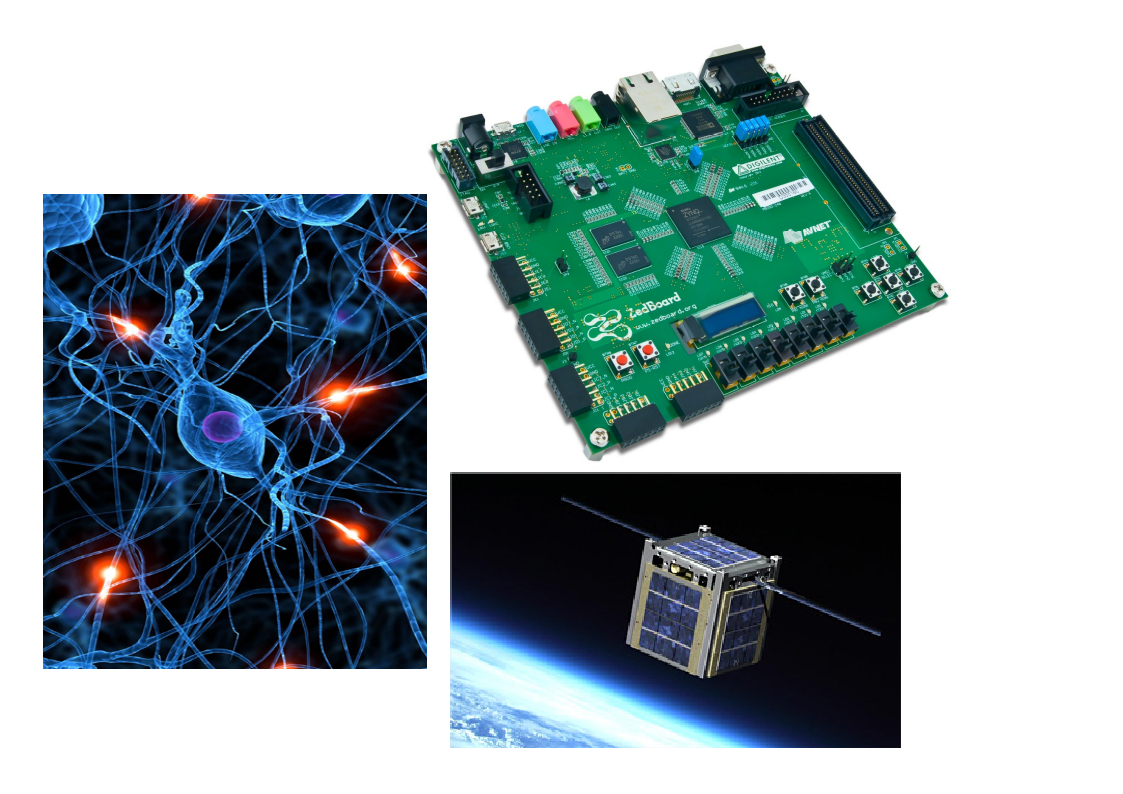
\includegraphics[width=\columnwidth,keepaspectratio]{figures/frontCover.png}
\vfill
\setlength{\tabcolsep}{0pt}


\makeatletter
\begin{tabular}{p{40mm}p{\dimexpr\columnwidth-40mm}}
Project Title: & \textbf{\@title} \\[12pt]
Student: & \textbf{\@author} \\[12pt]
CID: & \textbf{\cid} \\[12pt]
Course: & \textbf{\course} \\[12pt]
Project Supervisor: & \textbf{\supervisor} \\[12pt]
Second Marker: & \textbf{\secondmarker} \\
\end{tabular}
\end{titlepage}

\onehalfspacing

\begin{abstract}
Over the last decade, advancements in the design of Convolutional Neural Networks (CNNs) have led to significant improvements in the accuracy of image classification systems. A potential application of a CNN image classifier would be  processing data on board a satellite. In such a situation, with limited power and computational resources, it would be beneficial to make use of an FPGA in order to alleviate the resource demands of the computationally expensive CNN. However, FPGAs are sensitive to ionizing radiation, and at orbital altitudes, the high radiation environment can induce a variety of errors in the FPGA fabric, casting doubt on the suitability of a commercial FPGA for CNN applications in space.

This project implements an FPGA based CNN, and simulates radiation-induced errors. These results are analysed to determine the impact on the system’s performance. \hl{[The tests are yet to be performed, and as such, this part of the abstract is not yet completed.]} The implementation target platform is the ZedBoard Zynq-7000 ARM/FPGA SoC. The  hardware and software portions of the embedded system are both implemented  using the Xilinx SDSoC development environment.
\end{abstract}

\newpage

\renewcommand{\abstractname}{Acknowledgements}
\begin{abstract}
I would like to thank Dr Felix Winterstein for the enormous amount of help and guidance that he provided, particularly in the final stages of the project. I'm extremely grateful for the time he invested in helping me overcome obstacles and without his aid, the project would not have been completed. I would also like to thank Shane Fleming for allowing me to take advantage of the great work he put in to building the socDrawer, and for the assistance he provided in setting it up to run my experiments.
\end{abstract}

\newpage

\tableofcontents

\newpage

\section{Introduction}
\label{sec:Intro}


Inspired by the structure of the optical nervous system in animals, a neural network is made up of layers of artificial neurons that recognise certain features from the input data. The concept of an artificial neural network was first introduced in 1980 \cite{neocognitron}, and driven by increases in computing power and a growth in machine learning applications, neural networks have become very powerful tools. In the last decade, the development of Convolutional Neural Networks (CNNs) has lead to great advancements in image classification accuracy.

CNNs are a powerful Deep Learning tool that can be used to solve extremely complex computational problems. In particular, they have gained popularity in image classification applications \cite{ImageNetChallenge}. Other popular applications within machine vision include video classification, face detection, and optical text recognition. Neural Networks are being used in a wide range of other fields as well including speech recognition, natural language processing and text classification.

However, whilst achieving exceptional performance, CNNs are extremely computation and resource heavy. Typically, they will be implemented on large servers or on GPU based systems to accommodate the need for computational power. As a result, implementing them on embedded systems, which typically have very limited resources, presents many challenges. A promising solution to this problem is the use of an FPGA, which provide a very high computational efficiency with low power usage, in addition to other benefits.

Now suppose that the FPGA based CNN will be implemented on a satellite. In orbit, the satellite will be exposed to intense radiation, and as a result, errors will be produced on the radiation-sensitive FPGA. Before such a satellite can be designed and launched, it is important to know how these errors would affect the performance of the CNN, and if the CNN design could be modified to mitigate the impact of these errors. Therefore, the aim of this project is to implement a CNN on an FPGA-based system, and then to investigate the suitability of this system for space applications.

\subsection{Project Motivation}
\label{sec:Intro-ProjectMotivation}

CNNs are an extremely valuable and powerful tool in modern machine learning, with countless applications. One of these potential applications is on board a satellite orbiting the Earth, using a camera to gather image data. Currently, these images would have to be transferred to a terrestrial base station in order to be processed and analysed for information. On small satellites, power is limited, and the communications equipment does not have a great data capacity. Therefore it is expensive for the satellite to transfer full images to the base station. In addition to this, the link between the station and the satellite may only be available at certain points in the satellite’s orbit, and the channel capacity may be dependant on factors such as weather interrupting signals. 

In this scenario, the rate at which data can be gathered is heavily limited by the rate at which the data can be transferred to Earth. A way to alleviate this problem would be to implement a CNN on board the satellite. The CNN could discern the usefulness of an image and discard uninteresting data, saving the cost of transferring it to Earth. The CNN could even analyse the images and send only the results to Earth, eliminating the need to transfer the images altogether. 

However, implementing such a system is not without challenges. The aforementioned radiation induced errors can completely disrupt electronic devices, and FPGAs are particularly vulnerable. The impact of these errors, referred to as Single Event Upsets (SEUs), is discussed in more detail in Section \ref{sec:Background-FPGAsAndSpaceApplications-SEUs}. These errors pose a risk that must be investigated and assessed before the CNN satellite can be attempted. If it is found that the system is never going to be feasible, then the design and construction of such a system would be an avoidable waste of time and resources. This is the motivation behind this project.

\subsection{Target Platform}
\label{sec:Intro-TargetPlatform}


The hardware used in this project is a product from Xilinx called a Zedboard, a development board for the Zynq-7000 System On a Chip (SoC). This board was chosen because of its useful hardware features and its integrated support for valuable Xilinx proprietary tools. These tools include High Level Synthesis systems, SoC design tools and the Soft Error Mitigation IP core. The Zynq-7000 consists of Xilinx FPGA as its Programmable Logic(PL), and a dual-core Cortex-A9 ARM processor as its Processing System(PS) integrated together. Data transfer between these performed by the AXI4-Lite interface, which is discussed in more detail in Section \ref{sec:Design-PSnPL}.

The ARM processor facilitates easy control of the system with a Linux kernel. This is then able to run software and initiate hardware processes in order to perform computations. Software for the processor was designed using the Xilinx SDSoC development environment.

Vivado HLS was used to design and build a hardware block from C++ code. Then Vivado was used to integrate this hardware block into an complete hardware architecture, allowing it to be connected to and controlled by the software. This was then synthesised and the generated bitstream was used to configure the FPGA.

\subsection{Report Structure}
\label{sec:Intro-Structure}

\textbf{Section \ref{sec:Background} - Background:} In order to guarantee that the reader has the contextual knowledge required to understand the project, this section will High Level Synthesis, and CNNs. FPGA implementations of CNNs and the difficulties of using FPGAs in radiation-heavy environments will also be explored.\\
\\
\textbf{Section \ref{sec:ProjSpec} - Project Specification:} This section details the project requirements that should be met by the final system.\\
\\
\textbf{Section \ref{sec:Design} - Design:} The decisions taken in the design process are described and explained in this section. The high level design is described, as well important aspects of the low level design.\\
\\
\textbf{Section \ref{sec:Imp} - Implementation:} This section illustrate how the system was implemented, aiming to provide the reader with an understanding of the development process.\\
\\
\textbf{Section \ref{sec:Test} - Testing:} The testing methodology used to verify various components of the system is detailed in this section.\\
\\
\textbf{Section \ref{sec:Eval} - Evaluation:} The focus of this section is the result of the investigation, including an evaluation of the system's performance.\\
\\
\textbf{Section \ref{sec:Conclusion} - Conclusion and Future Work:} This section will summarize the results of the project, highlight areas for improvement and further work, and present concluding remarks.\\

\newpage

\section{Background}
\label{sec:Background}


This section will provide some details and information that will provide context to the project, and will be useful for understanding key concepts in the rest of the report. High Level Synthesis tools, the basics of machine learning, and CNN structures will be described. FPGA implementations of CNNs, and the issues surrounding the use of FPGAs in space will also be discussed.

\subsection{High Level Synthesis}
\label{sec:Background-HLS}

Typically, digital circuits on reconfigurable hardware architectures, such as FPGAs, are designed using a Hardware Description Language (HDL) such as Verilog or VHDL. While these methods allow the designer to have a great level of control over the system, and can produce extremely efficient designs, the designer is forced to specify functionality at a very low level of abstraction, controlling cycle by cycle behaviour. Use of HDL tools requires hardware expertise and, when designing a complex system, makes for a long and cumbersome development process. Additionally, a lack of specialist knowledge can lead to an extremely inefficient design.

High Level Synthesis (HLS) tools are a  solution to this problem. An HLS tool is a software application which can interpret the desired behaviour of code written in a programming language like C or C++, and generate an HDL implementation of that behaviour, allowing the designer to work at a higher level of abstraction. This means that a software engineer can create FPGA designs without having to build up hardware expertise, allowing them to utilise the speed and efficiency of hardware designs. It also benefits hardware engineers, allowing them to design the system more quickly and reliably, facilitating the development of more complex systems \cite{HLS}. Popular HLS tools include academic, open-source software like LegUp, and commercial tools like Catapult-C and Xilinx's Vivado. In this project, the embedded system will be designed using SDSoC from Xilinx, which utilises Vivado HLS to produce a configuration for the Programmable Logic in the Zynq SoC.

\subsection{Machine Learning}
\label{sec:Background-ML}

The core functionality of a machine learning system is to perform tasks on new, unseen data based on a large set of previously seen training data. The training data will be split up in to different classes and the system uses this training data to build up a model that predicts which class the new data best fits in to. This can be applied to many situations, such as classifying images, recognising speech patterns, or piloting a vehicle. Machine learning allows an electronic system to be put in a brand new situation and use past experience to make a decision.

A machine learning system takes an array of values as an input. If the input is a image, the vector values will represent pixels. This is done for a grayscale image by representing each pixel's intensity with an integer on a scale from 0, for a black pixel, to 255, for a white pixel. If the image is coloured, there will be three vector values for each pixel, with the brightness in red, green and blue in the pixel being represented as separate values. Parameters called weights are used to compare the input with the training data, and system will output a set of scores, which represent the likelihood that the input is a member of each class in the training data. The input is assigned the class with the highest score. 

The performance of such a system is based on a process called training.  Training is an iterative process, traditionally performed with the following method, called supervised learning. A piece of training data is fed through the system and is assigned a score at the output. The scores are compared with the expected results and the weights are adjusted according to the error. The process is repeated until the error is sufficiently small for each piece of data in the training data set. The best results are produced by training with a large set of data, with lots of variety within each class, e.g. images of the similar objects with different angles, lighting, etc.

\subsubsection{Linear Classifier}
\label{sec:Background-ML-LC}

One of the simplest types of machine learning structure is the linear classifier. These treat each value in the input vector as the position of the input in a separate dimension, with the length of the vector $N$ being the total number of dimensions. The linear classifier works by forming an $N$-dimensional space and dividing it up. The number of subspaces resulting from these class boundaries matches the number of classes that the classifier is trained to recognise, and the class boundaries are placed by the training process. New data is treated as a point in the $N$-dimensional space and is assigned the class of the subspace that it falls in to.

\begin{figure}[H]
\centering
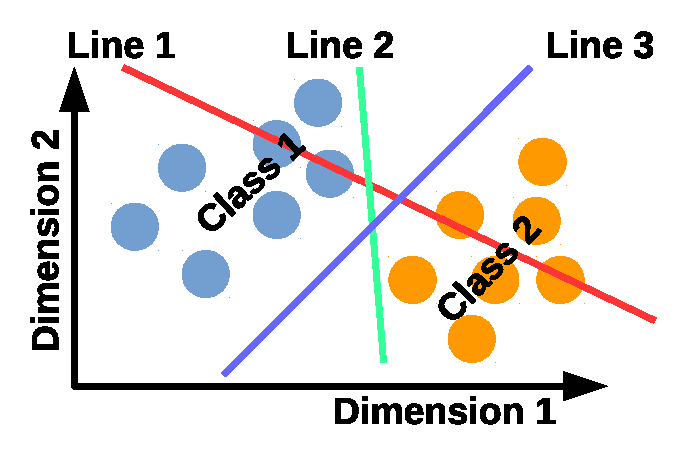
\includegraphics[width=0.5\textwidth]{figures/SVM.eps}
\caption{A linear classifier, with multiple class boundaries of differing quality shown}
\label{fig:SVM}
\end{figure}

Figure \ref{fig:SVM} shows this process taking place with two classes and a two dimensional input space. A good class boundary should separate the classes completely, and should find the maximum margin of separation, so that the chances of new data falling on the wrong side of the boundary is minimised. Clearly, Line 1 is a poor class boundary as the classes are not separated. Line 2 is acceptable, but only separates the classes by a small margin and is therefore is far from optimal. Line 3 is the best class boundary as it separates the classes with the largest margin, allowing a wider range of inputs to be correctly classified.

As previously stated, Linear Classifiers are a simple solution and are useful for fast classification, but have drawbacks associated with them. They are only designed as a binary classifier, discerning between only two problems. Algorithms exist to apply a binary classifier to multi-class problems, but these reduce the performance significantly. Traditional linear systems such as this are unable to accurately account for high levels of variation in inputs, which led to the development of non-linear machine learning systems, such as Neural Networks.

\subsubsection{Artificial Neural Networks}
\label{sec:Background-ML-NN}

Artificial Neural Networks are based on the structure of biological brains. A brain is made up of billions of interconnected building blocks called neurons. The structure of a neuron and an accompanying mathematical mode are shown in Figure \ref{fig:neuron}. Synapses act as the connections between neurons, supplying the dendrites with information. The dendrites act as an input, carrying the information to the cell body. The computation in the cell body is a weighted summation of the dendrite inputs, and the activation function determines the activation of the output neuron\cite{neuron}. Many activation functions exist in artificial models, but usually they define a threshold that must be surpassed by the computation result before it is passed on to the output, and these activation functions are the source of non-linearity in the network.

\begin{figure}[H]
\centering
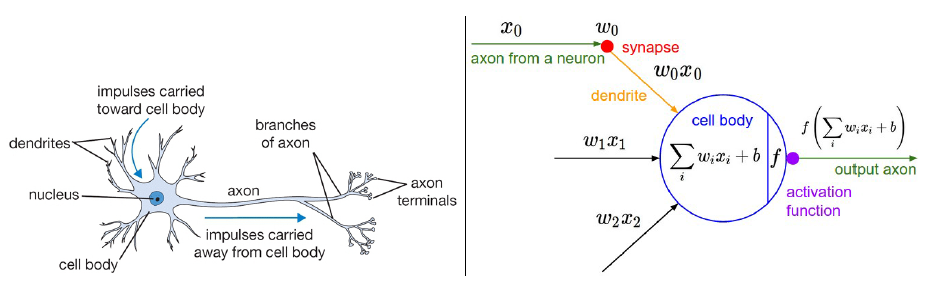
\includegraphics[width=0.9\textwidth]{figures/neuron.png}
\caption{A neuron, and a mathematical model of a neuron\cite{neuron}}
\label{fig:neuron}
\end{figure}

These neurons are connected together into a network as shown in Figure \ref{fig:ANN}. The neurons are arranged into layers, and connected to each neuron in the next and previous layers. The network has a layer for the input values and for the output values, and intermediate layers which are referred to as hidden layers since their only interaction is with the other layers. The number of hidden layers can vary, but has a big impact on how accurate the classification can be, and how many classes can be accurately classified. Deep networks with 10-20 layers have been shown to perform significantly better than shallow networks\cite{DeepNetworks}.

\begin{figure}[H]
\centering
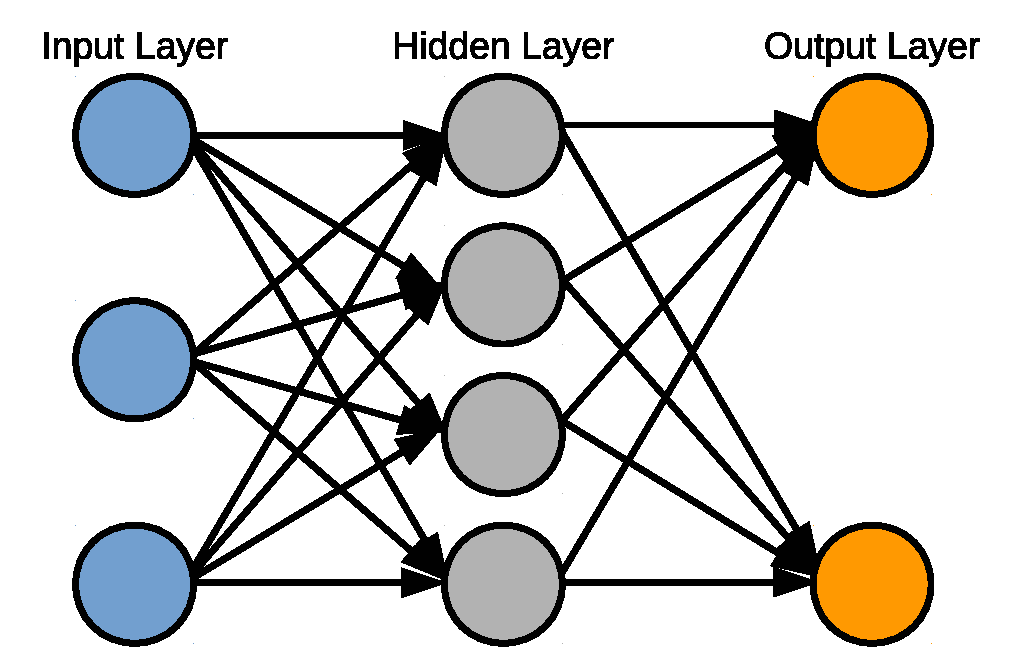
\includegraphics[width=0.5\textwidth]{figures/ANN.eps}
\caption{Simple Neural Network with one hidden layer}
\label{fig:ANN}
\end{figure}

Neural Networks are trained in a slightly different way to other machine learning systems, using a method called back-propagation. Inputs are propagated forwards through the network until the output is reached. The resulting output values are each compared against the desired values and an error value is calculated for each output neuron. The error values are then propagated backwards through the network and the weights of each neuron are adjusted accordingly. This process is repeated until the network is sufficiently trained.

\subsection{Convolutional Neural Networks}
\label{sec:Background-CNN}

CNNs are a specialised type of Neural Network, designed to be deep networks that model the visual perception of animals. They are usually designed to take images as inputs. The training of a CNN is often implemented on large servers with a significant computational capacity, with an enormous set of training data, or on a GPU when such a server is not available. For example, CNNs built for the ImageNet Large Scale Visual Recognition Challenge (ILSVRC) from 2012 to 2014 used a training dataset of approximately 1,281,167  images, grouped into 1000 classes\cite{ILSVRC}. In the case of the embedded FPGA platform, this project will only focus on implementing and utilising the inference process of a CNN, and not on the training process.

A typical CNN consists of a number of layers that run in sequence. Convolution, activation function, pooling, and fully connected layers make up a typical CNN model, with convolution and fully connected being the most important. Convolution and fully connected layers have parameters of called weights, which are set by the training process. These weights will determine which patterns each layer of the CNN will be activated by, and ultimately, what the CNN is able to recognise and classify. 

The first layer of a CNN reads an input image and outputs a series of feature maps. The input image will be three dimensional - the height and width of the image make up two dimensions, and colours make up the third layer. For an RGB image, the input will have a depth of 3. Then there will be convolution layers interspersed by activation function and pooling layers, which will make up most of the CNN. These layers will decompose the image into feature maps, varying from low-level features such as edges, lines, curves, etc., in the initial layers to high-level features in the deeper layers \cite{SudaFpgaAccelerator}. Each subsequent layer reads the feature maps generated by preceding layers and generates new feature maps at its output. Finally a classifier, consisting of at least one fully connected layer, reads the final feature maps and determines the probability of the input imaging belonging to each category of the training data. An example of a CNN model is shown in Figure \ref{fig:typicalCNN}.

\begin{figure} [H]
\centering
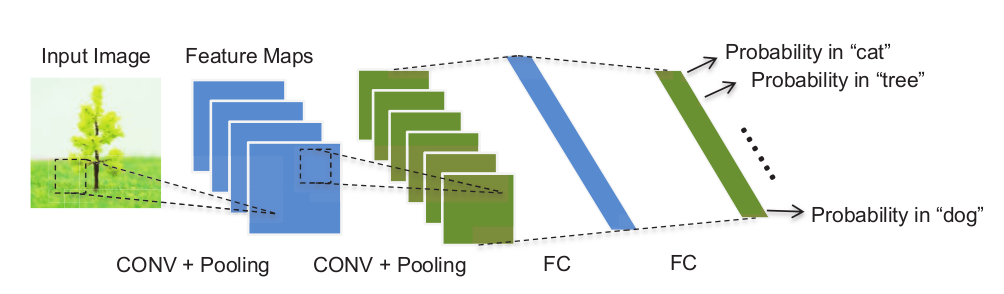
\includegraphics[width=0.9\textwidth]{figures/typicalCnn}
\caption{A typical CNN structure from the feature map perspective \cite{embeddedFpgaCnn} \label{fig:typicalCNN}}
\end{figure}

\subsubsection{Convolution Layer}
\label{sec:Background-CNN-Conv}

The convolution layer takes a series of feature maps as input and convolves with convolutional kernels to obtain the output feature maps. The simplest version of the convolution operation a involves 3-dimensional multiply and accumulate operation of $N_{if}$ input feature maps with $K\times K$ convolution kernels to get an output feature neuron value as shown in Equation \ref{eq:ConvLayer}
\begin{equation}
out(f_o,x,y)=\sum^{N_{if}}_{f_i=0} \sum^{K}_{k_x=0} \sum^{K}_{k_y=0} wt(f_o,f_i,k_x,k_y)\times in(f_i,x+k_x,y+k_y)
\label{eq:ConvLayer}
\end{equation}
where $out(f_o,x,y)$ and $in(f_i,x,y)$ represent the neurons at position $(x,y)$ in the feature maps $f_o$ and $f_i$, respectively and $wt(f_o,f_i,k_x,k_y)$ is the weights at position $(k_x,k_y)$ that gets convolved with input feature map $f_i$ to get the output feature map $f_o$ \cite{SudaFpgaAccelerator}.

Each position that the kernel takes corresponds to one output position and is referred to as an input region. This process can be thought of as the weights kernel scanning over the input feature map with, filtering each input region, and passing the result to the output. Many convolutions also include features called zero padding, adding layers of zeros around the input, and stride, moving the kernel over the input in steps. Zero padding can ensure that features on the edge of the feature map do not have a reduced contribution to the output, and stride reduces the computational cost of the layer by reducing the number of weights kernels needed, and reducing the dimensions of the output feature map.

\begin{figure} [H]
\centering
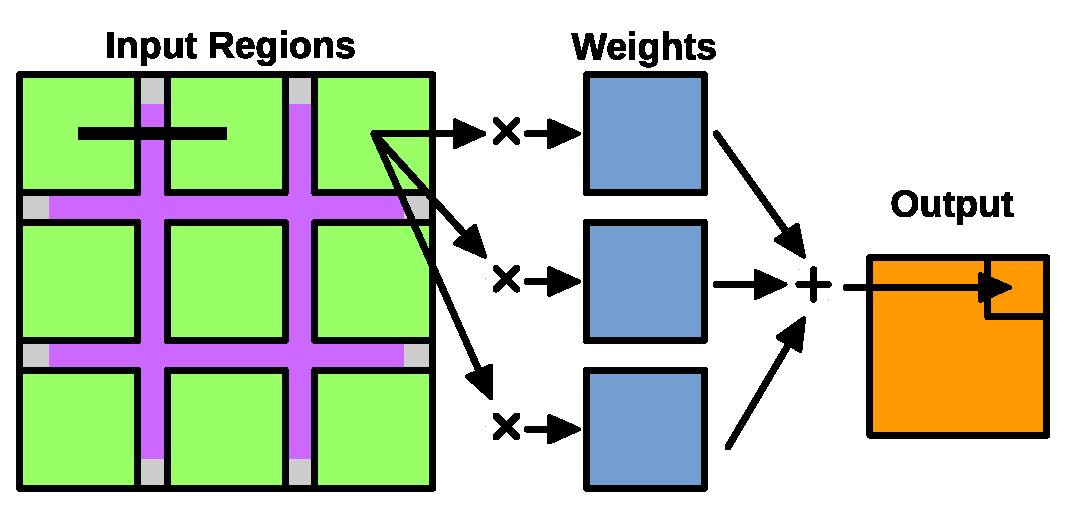
\includegraphics[width=0.9\textwidth]{figures/conv.eps}
\caption{A visualisation of a convolution computation for one output location}
\label{fig:conv}
\end{figure}

Figure \ref{fig:conv} shows a visualisation of the convolution operation. The input feature maps are shown on the left in purple, surrounded by grey zero padding. The green squares show the input regions, the positions of the weights kernel as it scans across the input. The element-wise product of the input region and the kernel is found and summed, and then added to the relevant output value. Each orange square in the output feature maps represents a single value. In this diagram, the input has two layers, and the output has three layers. It can be seen that the computation results for multiple input layers are added together to form the final output values. For multiple output layers, the computation process is repeated with new weights kernels. The number of weights is the product of the number of input layers and the number of output layers. Note that the diagram only depicts the computation for a single output location. The computation is repeated for every output location. 


\subsubsection{Activation Functions}
\label{sec:Background-CNN-Activation}

Convolution layers are followed by an activation function layer. This layer can be thought of as a decision, based on the output of the convolution layer, on to what extent each neuron in the next layer has been activated. The convolution layer output is a linear combination of the inputs and the weights at a position in the network, and role of the activation function is to produce a non-linear decision boundary. The commonly used activation functions in traditional neural networks are non-linear functions such as tanh and sigmoid, which require a longer training time in CNNs \cite{AlexNet}. Hence, Rectified Linear Unit (ReLU), defined as $y = max(x,0)$, has become the popular activation function among CNN models as it converges faster in training, and has less computational complexity than exponent functions in tanh and sigmoid, also aiding hardware design.

\subsubsection{Pooling Layer}
\label{sec:Background-CNN-Pool}


Spatial pooling or sub-sampling is utilized to reduce the feature dimensions as we traverse deeper into the network. As shown in Equation \ref{eq:Pool}, pooling computes the maximum of neighbouring $K\times K$ neurons in the same feature map, which also provides a form of translational invariance \cite{PoolAnalysis}. 
\begin{equation}
out(f_o,x,y)=\underset{0\geqslant (k_x,k_y)<K}{max}(in(f_o,x+k_x,y+k_y))
\label{eq:Pool}
\end{equation}

The pooling layer is sometimes computed by computing the average of each input region, but in this project only maximum pooling was used. Figure \ref{fig:pool} shows the operation of a max pooling layer graphically. The pooling layer is important as it reduces the dimensionality of lower-level features without losing important information, thus reducing the computational cost of the network \cite{SudaFpgaAccelerator}. A paper by J. Springenberg, A. Dosovitskiy, T. Brox and M. Riedmiller proposes an "all convolutional network" in which the pooling layers are eliminated by increasing the stride in some convolution layers without any reduction in performance\cite{AllConv}. Based on these results, pooling layers may soon stop appearing in new CNN architectures.

\begin{figure} [H]
\centering
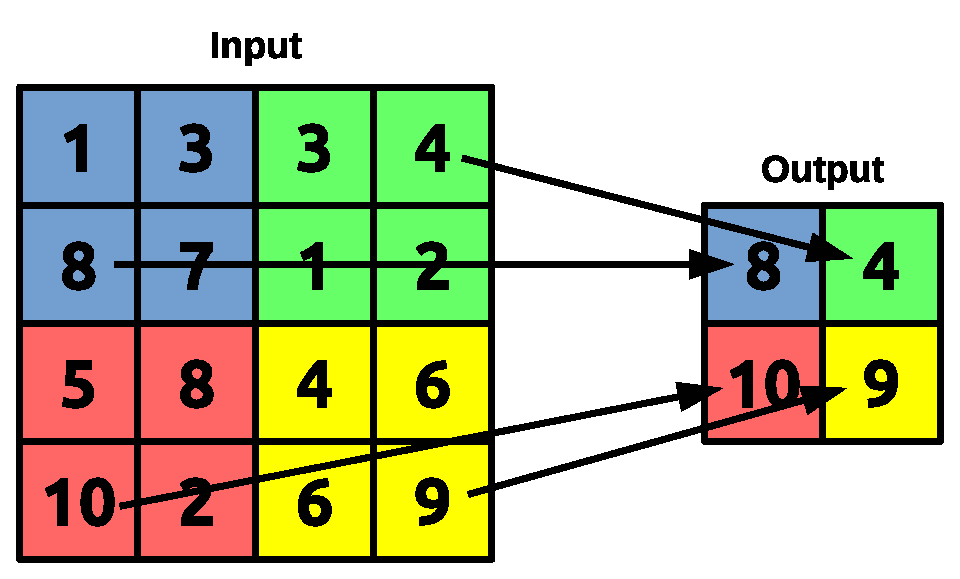
\includegraphics[width=0.5\textwidth]{figures/pool.eps}
\caption{A visualisation of the max pooling layer}
\label{fig:pool}
\end{figure}

\subsubsection{Fully Connected Layer}
\label{sec:Background-CNN-FC}


A fully connected layer is a classification layer where all the input features $(N_{if})$ are connected to all of the output features $(N_{of})$ through synaptic weights $(wt)$. These are at the end of the CNN and perform the final classification, based on the features that have been recognised by the rest of the network. Each output neuron is the weighted summation of all the input neurons, as shown in Equation \ref{eq:FullyConnected} \cite{SudaFpgaAccelerator}.
\begin{equation}
out(f_o)=\sum^{N_{if}}_{f_i=0}wt(f_o,f_i)\times in(f_i)
\label{eq:FullyConnected}
\end{equation}

This equation is visualised in figure \ref{fig:fc}. As the name suggests, every input neuron is connected to every output neuron and each connection has a unique weight. In this diagram, each arrow represents a multiplication with the corresponding weight. It can be seen that the fully connected is essentially the same as a layer of the standard artificial neural network described in \ref{sec:Background-ML-NN}. The outputs of the fully connected layer traverse through ReLU based activation function to the next fully connected layer or directly to a Linear Classifier as described in \ref{sec:Background-ML-LC}. The Linear Classifier will take the output feature map of the network use it to determine the scores for each class.

\begin{figure} [H]
\centering
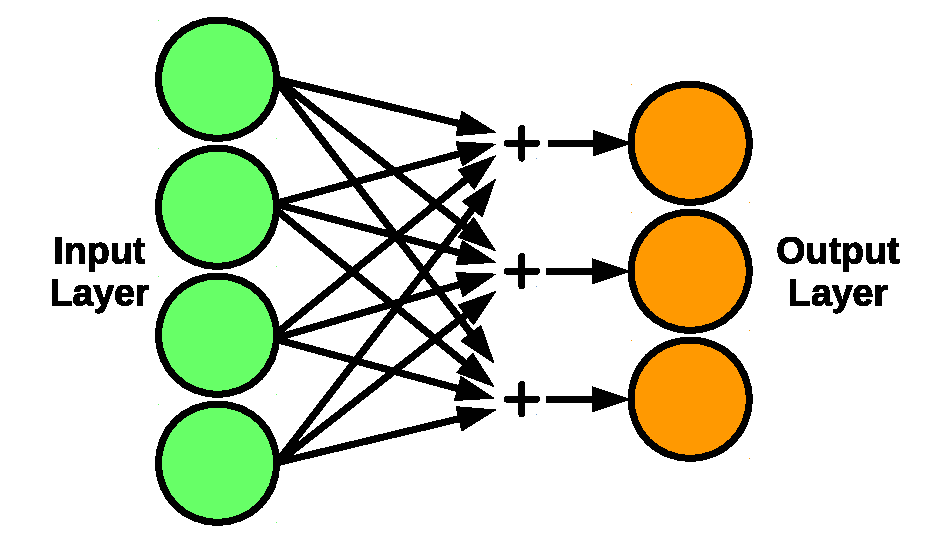
\includegraphics[width=0.5\textwidth]{figures/fc.eps}
\caption{Connections in a fully connected layer}
\label{fig:fc}
\end{figure}

\subsection{FPGAs and CNN Implementations}
\label{sec:Background-FpgaCnnImpl}


CNNs are computationally demanding and consume a lot of resources, and thus are difficult to implement on an embedded systems. FPGAs are the most promising platform for the implementation of an embedded CNN, due to their high computational efficiency and low power consumption. FPGAs are also more attractive than other digital hardware platforms, such as ASICS, because of their reconfigurability and fast development time, aided by HLS tools.

\subsubsection{Implementation Challenges}
\label{sec:Background-FpgaCnnImpl-Challenges}


One of the main challenges faced by FPGA implementations is memory bandwidth. A typical CNN model may have more than 60 million weights, which requires over 200MB of memory when represented with a 32 bit number. A standard commercial FPGA does not have enough on-chip memory to store this volume of data, so external memory must be utilised. Having to transfer this information to the FPGA can introduce a computational bottleneck. However, these weights are used in convolution layers multiple times. Thus, the system can be optimised by reducing frequent memory access. Chen et. al achieves this with a tiling method and dedicated buffers for data re-use. Another approach, is data quantization, which is discussed below. By quantizing the 32-bit floating-point weights into 16-bit fixed-point values, the pressure on the memory system can be alleviated. Suda et al. performed a study on the optimal precisions to balance accuracy and efficiency. It was found that the best choices were 8-bit precision for convolution weights, 10-bit precision for fully connected weights, with less than 1\% compared accuracy loss compared to full precision weights \cite{SudaFpgaAccelerator}.

\subsubsection{FPGA CNN Accelerators}
\label{sec:Background-FpgaCnnImpl-Accel}


An FPGA implementation of a CNN, intended to improve the speed and efficiency of the CNN computation, is referred to as an FPGA CNN accelerator. Most research into FPGA CNN accelerators has focussed on using hardware to accelerating the computation of the convolution layers. These layers typically make up around 90\% of the CNN's computational workload. The multiply and accumulate nature of the convolution layer's operation makes them ideal candidates for hardware acceleration, as FPGAs are able to perform these operations with great efficiency. 

FPGAs also provide flexibility to implement the CNNs with limited data precision \cite{SudaFpgaAccelerator}. Many CNN accelerators use 16-bit fixed-point numbers instead of floating-point numbers to represent weights and data \cite{ZhangFpgaAccelerator}\cite{ChenFpgaAccelerator}\cite{FarabetFpgaAccelerator}, especially because FPGAs. Using a shorter, fixed-point data representation can make significant reductions to the memory footprint and the use of computational resources. The CNN's data must be quantised in order for the fixed-point implementation to work, which will introduce a quantization error into the result. However, Chen et al. showed that using a 16-bit fixed-point implementation rather than a 32-bit fixed-point implementation only added an extra 0.26\% to the error rate when using the MNIST dataset.

\subsection{FPGAs and Space Applications}
\label{sec:Background-FPGAsAndSpaceApplications}

\subsubsection{Single Event Upsets}
\label{sec:Background-FPGAsAndSpaceApplications-SEUs}

Electronic circuits are sensitive to high-energy ionizing radiation, which can induce errors called Single Event Upsets (SEUs) \cite{SeuTutorial}. In space, this is a particular problem. The radiation shielding provided by the Earth's magnetosphere, and enjoyed by systems at lower altitudes, is no longer present, leaving systems open to radiation from a  variety of sources. A voltage pulse from an SEU can cause errors including altering digital values. SEU induced voltage pulses are problematic for all circuits in space, but the nature of reconfigurable circuits means that they are particularly vulnerable. These SEUs are typically manifested as a bit flip in a memory cell or a transient logic pulse in combinational logic. Habinc et al. describes three main categories of SEU \cite{SuitabilityGaisler}.

The first category is the configuration upset. FPGAs are configured by loading the configuration bitstream into an internal configuration memory. This memory controls the configurable logic elements and how they connect together. A configuration upset occurs when an SEU alters a value in the configuration memory, and thus changes the function of the configuration. 

The second category is the functional upsets in user logic are SEUs within the FPGA's logic. The FPGA's user logic cannot be tested through a read back of the configuration memory, because the logic contents will change as part of normal operation. These errors can cause transient glitches in combinatorial logic, and can upset sequential logic where the state of the system is vital to its function \cite{FTripleMR}.

The final category is the architectural upset. This is when an SEU occurs in the control elements of the FPGA, e.g. the configuration circuits or reset control \cite{SuitabilityGaisler}. This can have an enormous range of consequences. For example, an SEU in the reset control could cause the FPGA to be unintentionally reset and all state information would be lost due to the FPGA being reconfigured.

Architectural upsets are outside the scope of this project, but configuration and functional upsets will be investigated. This is explained in more detail in Section \ref{sec:ProjSpec-TestSpec}.

\subsubsection{SEU Mitigation Techniques}
\label{sec:Background-FPGAsAndSpaceApplications-Mitigation}

As a result of the problems that can be caused by SEUs, many techniques have been developed to mitigate the impact of SEUs in space. A few popular design techniques for overcoming SEU errors are described below. Although this is outside the scope of the project, some of these techniques could potentially be used to increase the SEU resilience of the FPGA CNN implementation.

A very effective way of detecting configuration upsets is to read back and verify the configuration memory of the FPGA. As long as the external memory holding the bitstream is uncompromised, any discrepancies caused by SEUs can be detected and corrected \cite{SuitabilityGaisler}. The disadvantage of this method is that any sequential logic within the FPGA will lose all state information.

Functional Triple Modular Redundancy is another popular method of mitigating SEU errors \cite{FTripleMR}. This involves making three copies of a given design within the FPGA fabric, and having them 'vote' on the result through a combinatorial circuit. This is very effecting at reducing the error rate from combinatorial and user upsets, as two of the three circuits need to be compromised in the same way in order for a false result to be given as the output of the system.

Radiation hardening is the act of physically making a chip less susceptible to radiation, typically by encasing it in a substance that will shield the internal electronics \cite{RadHardFpga}. Many FPGA vendors sell radiation hardened versions of their products, and it should greatly reduce the impact of SEUs, but it is often a very expensive solution due to the cost of the 'rad hard' hardware.

\subsubsection{Soft Error Mitigation (SEM) Core}
\label{sec:Background-FPGAsAndSpaceApplications-SEM}

The Soft Error Mitigation core is a Xilinx Intellectual Property (IP) core that can be used to detect, correct and classify SEUs. More importantly, it also provides error injection functionality\cite{SEM}. Once added to a hardware system, it is able to emulate SEUs, allowing the evaluation of the SEU mitigation capabilities of a hardware design. This is a valuable feature as it allows a much cheaper, safer and more controlled method of testing the system than using a radiation source to induce the errors. 

\newpage

\section{Project Specification}
\label{sec:ProjSpec}

In this section, the requirements and design specifications captured during the planning of the project will be discussed. The requirements will be divided into two set of functionalities - those that are necessary for the project to be considered a success, and those that are not essential but would greatly enhance the system and the results gathered - and briefly described. Following this, the testing and evaluation specifications are laid out and discussed.

\subsection{Necessary Functionality}
\label{sec:ProjSpec-Necessary}

\subsubsection{Running On Zedboard}
\label{sec:ProjSpec-Necessary-Zedboard}

The system should be able to run on the target platform, described in Section \ref{sec:Intro-TargetPlatform} as the Xilinx Zedboard. The compilation of the program will produce an executable file in either .bin or .elf format, and this should run on the hardware platform, either printing a stream of output that can be read through a serial connection or storing the results in a file .log or .txt to be read later.

\subsubsection{Software and Hardware Split}
\label{sec:ProjSpec-Necessary-split}

An important part of the design is to intelligently spit the processing responsibilities between the hardware and software of the Zynq-7000. The various parts of the system should be analysed and compared to determine which parts are more suitable for hardware acceleration, and which parts are more suitable for software implementation.

\subsubsection{Convolution Layer Implemented in Hardware}
\label{sec:ProjSpec-Necessary-Conv}

As previously explained in Section \ref{sec:Background-FpgaCnnImpl-Accel}, the convolution layer represents the biggest portion of the computational workload, and is thus the primary focus of the examination. It is therefore important that the convolution layer is at least partially implemented in hardware to allow testing with the SEM core. By analysing how the convolution layer is affected by SEUs, information about the effects on the rest of the network can be inferred.

\subsubsection{SEM Core Integrated into Design}
\label{sec:ProjSpec-Necessary-SEM}

In order to perform the SEU emulation with the SEM core as described in Section \ref{sec:Background-FPGAsAndSpaceApplications-SEM}, it is necessary to integrate the SEM core into the the digital hardware design. 

\subsection{Desirable Functionality}
\label{sec:ProjSpec-Desirable}

\subsubsection{Full CNN Implementation}
\label{sec:ProjSpec-Desirable-SEM}

It would be desirable for a full CNN model to be implemented. With this in place, it would bee possible to run 

\begin{itemize}
\item Full CNN implemented, able to process and classify images with reasonable accuracy
\item System is optimised to run as efficiently as possible
\end{itemize}

\subsection{Testing Specification}
\label{sec:ProjSpec-TestSpec}

\begin{itemize}
\item Compare control results against pure software implementation to verify correctness
\item Where numerical approximations are required, trade-off must be justifiable
\end{itemize}

\subsection{Evaluation Specification}
\label{sec:ProjSpec-EvalSpec}

\begin{itemize}
\item Analyse SDSoC's estimate of hardware resources used, as well as actual resources used.
\item Compare computation time/performance against those in literature
\item If applicable, compare CNN accuracy to those in literature
\item Assess impact of SEUs with Failure In Time measurement
\end{itemize}

\newpage

\section{Convolutional Neural Network
 Design}
\label{sec:Design-Network}

\hl{TODO}

\begin{itemize}
\item Describe Network organisation and design (If full network is implemented)
\item Describe Caffe, Justify use as basis for design (pre-trained network models, etc)
\item mention blobs
\end{itemize}

\subsection{Data Objects}
\label{sec:Design-Network-Blobs}

In order for data to be easily processed by network layers, a class called \lstinline|DataMemory| was created. This is a simple wrapper around dynamically allocated memory that provides homogeneous storage of all data in the network. The data is accessed through functions called \lstinline|getConstData| and \lstinline|getMutableData|, which both return a pointer that can be used to access the data as an array. A \lstinline|const| pointer is returned by \lstinline|getConstData| for situations where the memory is only going to be read, and \lstinline|getMutableData| returns a normal pointer which can be used to read and write values to and from the memory space.

In order to make a universal, easily used data handler, the aforementioned \lstinline|Blob| class was created. This class acts as a wrapper around \lstinline|DataMemory| instances, and is used to store all data passing through the software portions of the network, including the weights data for convolution and fully connected layers. Blobs are given four dimensions (batch number, depth, height and width) and allow the stored data to be accessed as a four dimensional matrix of data, as opposed to a flat array. Most blobs would only use three of these dimensions, but weights blobs in convolution and fully connected layers use four layers. Additionally the fourth dimension allows multiple sets of input data to be propagated through the network together. This is referred to as batch processing. The Blob class also includes useful functions that simplify data handling, such as a \lstinline|count| function that returns the length of the data stored, and the \lstinline|CopyFrom| function that copies data from one blob to another. To keep the layer designs as simple as possible, the layers were designed to accept only square blobs as inputs and outputs. Therefore when describing a blob, "size" refers to both the height and width of the blob.

\subsection{Layer Design}
\label{sec:Design-Network-Layers}

Each layer type was implemented as a class, which provided several benefits. Every layer would be self contained, with all functions and data related to the class being easily accessible. The class data could also be protected from being changed in an unintended way by storing information in private variables, and allowing external access to the data only through dedicated functions that will not misuse it. Finally, using classes allows multiple, identical instances of the same layer types to be easily created.

In addition to multiple version of the same layers types, several very diverse layer types are required for a CNN to be properly implemented. If these were all implemented in vastly different ways, each with a unique interface for external code, setting up and running the network would be challenging, if not impossible. Such a network would be very difficult to control automatically, and the interaction with each individual layer would likely have to be hard coded. 

To overcome this problem, a class template was implemented for the network layers. A class template is a structure that defines a family of classes, providing a standardised set of functions and variables that will be inherited by all classes that use the class template as a base. The \lstinline|Layer| base class is therefore used to define three main functions that create an interface for the layer. These functions have different purposes and perform varying tasks depending on the layer, so these functions do not define any of the layer functionality, but define an interface and usage is standardised for every layer in the network. Each of these functions takes pointers to the top and bottom Blobs of the layer as inputs, as shown in Figure \ref{fig:layer}. With a small extension, it would not be difficult to implement layers that could handle multiple top and bottom Blobs, but this addition is unnecessary to compute the VGGnet CNN model, and was rejected in favour of keeping the implementation as simple as possible.

\begin{figure} [H]
\centering
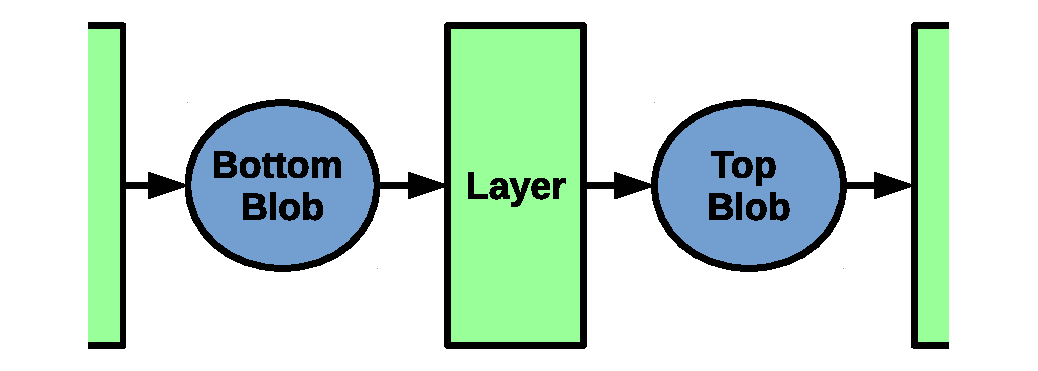
\includegraphics[width=0.75\textwidth]{figures/layer.eps}
\caption{A layer within the network structure, showing the top and bottom Blobs and their respective DataMemory objects}
\label{fig:layer}
\end{figure}

The \lstinline|LayerSetUp| function is run after the layer is originally constructed. Each layer class has a constructor that will initialise most of its parameters when a layer instance is created, but sometimes of these parameters are dependant on the shape of the bottom Blob. These parameters are then set by the \lstinline|LayerSetUp| function. This function also performs a sanity checks on the layer parameters to ensure that nothing is amiss.

The \lstinline|Reshape| function is run after \lstinline|LayerSetUp|. As the name suggests, it reshapes the top Blob to match the bottom Blob. A ReLU layer must produce an output of the same dimensions as the input, while a convolution layer's output is determined by a combination of the input size and kernel size, and the padding and stride parameters, but in every layer type, the output shape is a critical part of the layer's operation. This function therefore adjusts the top Blob so that the layer operates correctly.

The most important function in this interface is \lstinline|Forward|, which is run last and computes the output of each layer as described in Section \ref{sec:Background-CNN}. This simple interface allows a set of input data to be run through the entire network with a simple \lstinline|for| loop that iterates through the layers and uses the top Blob of a layer as the bottom Blob of the next layer until the final layer output is calculated.

\subsection{Convolution Layer}
\label{sec:Design-Conv}

The convolution layer is the most important layer in this network model for the purposes of this project, as it is where the bulk of the computation takes place, and is therefore most likely to be disrupted by SEUs. Therefore, this part of this layer had to be implemented in hardware to investigate the effects. First, two approaches to performing the convolution were implemented in software and compared. The more intuitive approach uses nested \lstinline|for| loops to iterate through the dimensions of the weights, inputs, and outputs and compute the results incrementally. The other approach reshapes the input and weight data, and performs the convolution in one large matrix multiplication. Once implemented and compared, it was clear that the intuitive approach was much more suitable for an FPGA implementation.

\subsubsection{Matrix Multiplication Method}
\label{sec:Design-Conv-MM}

The matrix multiplication method requires the data to be in a specific shape. Thus, the data is flattened and organized into a matrices. In this approach, the weights kernels are considered to be three dimensional, where the height and width are given by the kernel size, and the depth is given by the depth of the input feature map. The each three-dimensional weights kernel is flattened into a row and the each row is stored sequentially. Thus the result is an $M \times K$ matrix where $M$ is the number of weights kernels, and $K$ is the volume of an individual kernel. If the weights are stored sequentially in memory, this reshaping process can be done without copying any data to new locations. In such a situation, it is a simple case of changing how the memory will be accessed, by setting the depth and height of the weights Blob to 1, and the Blob width to $K$.

Then the input feature map is considered in terms of input regions, i.e. each area that will be multiplied with weights kernels. The size of these regions matches the weights kernel, and the number is dependent on the input size, kernel size, padding and stride.  These input regions are flattened and stored as columns. However, this is not as simple as changing the data access. If the convolution has padding, the input regions may contain extra zeros. Additionally, the stride and kernel size may result in input regions are overlapping or are not continuous. Therefore, each input region is individually mapped and copied from the input data into columns. This forms a $K \times N$ matrix, where $K$ is the volume of an input region, and $N$ is the number of input regions in the input feature map.

\begin{figure} [H]
\centering
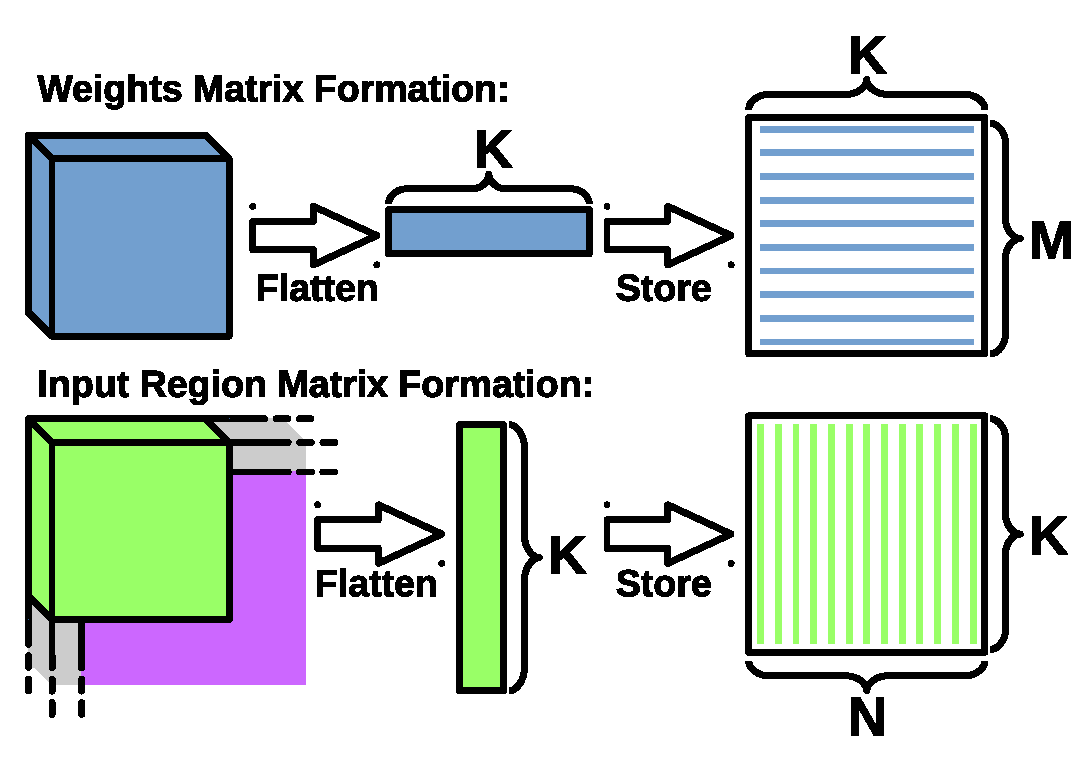
\includegraphics[width=0.75\textwidth]{figures/im2col.eps}
\caption{A visualisation of the reshaping process} 
\label{fig:im2col}
\end{figure}

Figure \ref{fig:im2col} shows a visualisation of the reshaping process. The weights data is shown in blue, and the input region data is shown in green, embedded in a purple feature map with grey padding. Once the matrices are formed, the output of the convolution is then found with \( \mathbf{C} = \mathbf{A}\times\mathbf{B}\), where $\mathbf{C}$ is the output matrix, $\mathbf{A}$ is the weights matrix, and $\mathbf{B}$ is the matrix of input regions. In order for this computation to be valid, it should be clear that the volume of an input region is the same as the volume of a kernel. By changing the output Blob dimensions, the $M \times N$ output matrix can be treated as feature map with depth $M$, equal to the number of weights, and width and height that give a product $N$, equal to the number of input regions.

By reducing the convolution to a single matrix multiplication, the algorithm can take advantage of a software library called Basic Linear Algebra Subprograms, or BLAS. This can bring significant performance improvements, as the BLAS library can provide highly optimised functions for a given platform. One such function is called \lstinline|gemm()|, and performs a general matrix multiplication, $\mathbf{C} \gets \alpha\mathbf{A}\mathbf{B} + \beta\mathbf{C}$, where $\alpha$ and $\beta$ are constants. By setting $\alpha = 1$ and $\beta = 0$, the \lstinline|gemm()| function can be used to compute the output of the convolution. This method is ideal for a software implementation of the convolution that will not be running on an embedded system. However, the weights matrix and input matrix will both be occupy a lot of memory in most practical CNNs, and a typical FPGA will not have enough on-chip memory to perform the entire convolution at once. This can be mitigated by breaking the matrix multiplication down into individual row and column multiplications, but the process of moving the input regions to a new memory space will be expensive in terms of both computational cost and memory footprint, so it is not well suited for an embedded system.

\subsubsection{Tiled Convolution Method}
\label{sec:Design-Conv-TC}

Directly interpreting the convolution algorithm as described in \ref{sec:Background-CNN-Conv}, the pseudo-code in Code \ref{code:conv-initial} can be formed. This code iterates through the rows, columns and depth layers of the output, as well as the rows and columns of the weights kernels and the depth layers of the input. The input row and column for the given kernel and output locations are found in lines 6 and 8. The formula $inIndex = stride * outIndex + kernelIndex - zeroPadding$ is used to calculate the input index in the height and width dimensions. In the centre of the loops, the value in the output feature map is incremented by the product of the corresponding weight and input values, but if the input location is in a padded region, the input value is 0. Therefore, the output only changes when the input is not in padding. It can be noted that this pseudo-code is functionally identical to the Matrix Multiplication method, except that the computation is performed value at a time, and the input data is not moved to a new location in memory.

\renewcommand{\lstlistingname}{Code}
\begin{lstlisting}[caption=Basic Convolution, label=code:conv-initial, language=C, float=ht]
for(outRow=0; outRow<OutputHeight; outRow++){
	for(outCol=0; outCol<OutputWidth; outCol++){
		for(outDep=0; outDep<OutputDepth; outDep++){
			for(inDep=0; inDep<InputDepth; inDep++){      
				for(kernelRow=0; kernelRow<KernelHeight; kernelRow++){        
					// calculate inRow
					for(kernelCol=0; kernelCol<KernelWidth; kernelCol++){          
						// calculate inCol
						if( input is not in padded area ){
							output[outDep][outRow][outCol] +=
								weights[outDep][inDep][kernelRow][kernelCol] *
								input[inDep][inRow][inCol];
}}}}}}}
\end{lstlisting} 

Put straight on to an FPGA, this algorithm will require the entire input feature map and all of the weights kernels to be loaded onto the FPGA at once, which is not feasible for a typically sized convolution layer. However, Zhang et al. describes a method of tiling the data so that the convolution can be performed in chunks and is therefore suitable for FPGA computation. The code is split into two parts. Code \ref{code:conv-sw}  is responsible for managing the data tiling and loading the tiles of data into the computation kernel. Code \ref{code:conv-hw1} shows the computation kernel that performs the tiled convolution computation.

Code \ref{code:conv-sw} iterates through the same dimensions as the outer four loops in the Code \ref{code:conv-initial}, but is incremented by the tile size for that particular dimension. If an appropriate set of tile sizes can be found, the tiling approach can allow convolutions of various sizes to be performed using the same kernel, which leads to very efficient use of FPGA resources. Tiling also allows the computation to be performed using multiple hardware kernels in parallel.

\renewcommand{\lstlistingname}{Code}
\begin{lstlisting}[caption=External Data Transfer, label=code:conv-sw, language=C, float=ht]
for(outRow=0; outRow<OutputHeight; outRow+=outRowTileSize){
	for(outCol=0; outCol<OutputWidth; outCol+=outColTileSize){
		for(outDep=0; outDep<OutputDepth; outDep += outDepTileSize){
			for(inDep=0; inDep<InputDepth; inDep += inDepTileSize){
				LoadInputTile();
				LoadWeightTile();
				LoadOutputTile();
}}}}
\end{lstlisting} 

The computational kernel shown in Code 3 iterates through the tile and performs the convolution for the tiled region. The code is nearly identical to Code 1, but is performed only on one tile of data. Section \ref{sec:Imp-Optimisations} describes how this kernel can be further optimised.

\renewcommand{\lstlistingname}{Code}
\begin{lstlisting}[caption=Computational Kernel, label=code:conv-hw1, language=C, float=ht]
for(outRow=outRowTileStart; outRow<outRowTileEnd; outRow++){
	for(outCol=outColTileStart; outCol<outColTileEnd; outCol++){
		for(outDep=outDepTileStart; outDep<outDepTileEnd; outDep++){
			for(inDep=inRowTileStart; inDep<inDepTileEnd; inDep++){
				// calculate inRow
				for(kernelCol = 0; kernelCol<KernelWidth; kernelCol++){
					// calculate inCol
					if( input is not in padded area ){
						output[outDep][outRow][outCol] +=
							weights[outDep][inDep][kernelRow][kernelCol] *
							input[inDep][inRow][inCol];
}}}}}}
\end{lstlisting} 

Because tiling allows for the data space to be efficiently broken down into parts, this convolution method avoids being limited by the memory capacity is much more suitable for hardware implementation. Additionally, a computational kernel of the same size can be reused for different convolution sizes. This eliminates the need to have multiple convolution hardware blocks of different sizes implemented independently on the FPGA, saving valuable hardware resources. Therefore, this algorithm was chosen to be implemented in HLS.

\subsubsection{Layer Setup}
\label{sec:Design-Conv-Setup}

To set up the layer, values for zero padding, output depth, stride and kernel size parameters are provided. Using these parameters and reading the dimensions of the input, the output height and width are calculated using Equation \ref{eq:ConvOutSize}.
\begin{equation}
outputSize = inputSize + 2 \times zeroPadding - kernelSize) / stride) + 1
\label{eq:ConvOutSize}
\end{equation}

If $outputSize$ is not an integer, then combination of the input size, zero padding, kernel size, and stride is not valid to perform a convolution. This result is checked, and then the output Blob is reshaped to have the dimensions $(outputDepth \times outputSize \times outputSize)$. Finally the weights blob is reshaped to have dimensions $(outputDepth \times inputDepth \times kernelSize \times kernelSize)$ and is filled with zeros to be initialised.

\subsection{Fully Connected Layer}
\label{sec:Design-FC}

The fully connected layer is the only layer apart from the convolution layer with a large computational footprint. The fully connected layer does	 perform as many computations, but has a larger memory footprint, partly because no weights are re-used between computations. It was hoped that the impact of SEUs on this layer would be investigated as well, so a hardware implementation was designed. Similarly to the convolution layer, two software algorithms were implemented and compared before deciding on  version to implement in hardware. 

\subsubsection{Vector-Matrix Multiplication Method}
\label{sec:Design-FC-MM}

Each output neuron of the fully connected Layer, is assigned a weighted sum of the outputs of every neuron in the input layer, as described in Section \ref{sec:Background-CNN-FC}. This can be computed by considering the input values as a vector and the weights as a matrix, and performing a vector-matrix multiplication. The input is given as a vector of $K$ values. Fully connected layers produce vectors as outputs, but the outputs of other layer types is flattened to create this input vector. The weights are given as a $K \times N$ matrix, where $N$ is the number of output neurons. The output is then found with \( \mathbf{C} = \mathbf{A}\times\mathbf{B}\), where $\mathbf{C}$ is the output vector of length $N$, $\mathbf{A}$ is the weights matrix, and $\mathbf{B}$ is the vector  of input values. 

If the network computation is being performed in batches (i.e. multiple sets of input data are being propagated through the network together), every input set in the batch can be computed at once by combining the input and output vectors. This results in matrices of size $B \times K$ and $B \times N$ for the input and output respectively, where $B$ is the number of input sets in the batch.

The vector-matrix multiplication is the intuitive solution to computing the fully connected layer, as the computation follows the description of the fully connected layer's operation - each output value is a weighted sum of the inputs. By treating the vectors as matrices with size $1$ in one dimension, the vector-matrix multiplication is evaluated in the same way as a standard matrix-matrix multiplication. Conveniently, this means that the method will work for batches of data without any modifications beyond changing the matrix dimensions. As described in Section \ref{sec:Design-Conv-MM}, this method of computation can take advantage of the \lstinline|gemm| function to increase performance. Once again, this is ideal for a software implementation, but is not suitable for an embedded system with limited computational resources.

\subsubsection{Dot Product Convolution Method}
\label{sec:Design-FC-Conv}

An alternative method of computing the fully connected layer is to compute it with a convolutional kernel. For this, we consider the inputs as a vector of length $N_{if}$. The weights are divided into $N_{of}$ vectors of length $N_{if}$, where $N_{of}$ is the length of the output, and one vector is assigned to each output feature. Equation 4 shows the formula for computing one output value in the fully connected layer. This is equivalent to a dot product of $in$, the input vector, and $wt_{f_o}$, the weights vector corresponding to the output feature. 
\begin{equation}
out[f_o] = \sum^{N_{if}}_{f_i=0} wt_{f_o}[f_i]\times in[f_i] = wt_{f_o} \cdot in
\label{eq:DotProd}
\end{equation}

The next thing to consider is how to perform a convolution on these flattened layers. As previously explained, the convolution operation scans a weights kernel over the input and at each position, an output value is assigned the sum of the element-wise product of the weights kernel and the input region. Equation \ref{eq:FlatConv} shows a formula for finding the convolution with a flattened input and a flattened weights kernel stored in a vector of length $K$, using $zeroPadding = 0, stride =1$
\begin{equation}
(wt*in)[n] = \sum^{K}_{k=0} wt[k]\times in[n + k - 1]
\label{eq:FlatConv}
\end{equation}

The size of the convolution output is equal to the number of input regions that the kernel scans over. Thus, by setting $K = N_{if}$, convolution will produce only one value and Equation \ref{eq:ConvDotProd} shows how the formula reduces to a dot product\cite{fc2conv}. As shown in Equation \ref{eq:DotProd}, the dot product is equivalent to finding the output value of a fully connected layer. Therefore, by setting the size of the convolution kernel to match the size of the input, we can compute a fully connected layer with the convolution computation.
\begin{equation}
(wt*in)[n] = (wt*in)[1] = \sum^{N_{if}}_{k=0} wt[k]\times in[1 + k - 1] 
= \sum^{N_{if}}_{k=0} wt[k]\times in[k] = wt \cdot in = out[f_o]
\label{eq:ConvDotProd}
\end{equation}

As discussed in section \ref{network structure}, VGG net consists of five sets of convolution layers followed by three fully connected layers. Therefore, the convolution-based fully connected layers will have two kinds of inputs. The bottom of the layer will be either the output of the convolutional part of the network or the output of another fully connected layer. In order to form the dot product, the size of the weights kernel must match the size of the input blob. At the end of the convolutional part of the network is a pooling layer that produces 512 different $7 \times 7$ feature maps at its output. Therefore, the first fully connected layer must use a $7 \times 7$ weights kernel. The fully connected layer produces a vector of values at its output. Therefore, any fully connected layers after the first on will treat their input as a set of $1 \times 1$ feature maps and will have a matching kernel size. In the VGGNet model, this applies to the final two layers.

A convolution is an ideal way to compute the result because the fully connected layer can be easily computed in uniform chunks, perfect for FPGA computation. In addition, the convolution layer has already been designed for the convolution layer, and any optimisations implemented in the design of the convolution layer can improve the performance of the fully connected layer with no extra work. Therefore, this method was selected to be implemented in hardware.

It is important to note that although they are both valid ways of calculating the result, the Vector-Matrix Multiplication and Dot Product methods use the weights in a different order, and one method cannot use weights trained for the other method without adjusting the order in which the weights are accessed. This problem is overcome by treating the weights as a matrix as described in the Vector-Matrix Multiplication method and using the transpose of this matrix in computations. The Caffe framework uses the Vector-Matrix Multiplication method to compute the results of the fully connected layer, so the Dot Product method implementation was modified to access the weights as if they were transposed. In doing this, consistency with the Caffe framework could be maintained, allowing the network to continue using pre-trained weights from Caffe's model zoo.

\subsubsection{Layer Setup}
\label{sec:Design-FC-Setup}

The only input parameter required for setting up the fully connected layer, apart from the input blob, is the output length. The weights blob is given the dimensions $(outputLength \times inputLength \times inputSize \times inputSize)$ and the output blob is reshaped to be a vector of length $outputLength$. 

\subsection{Rectified Linear Unit Layer}
\label{sec:Design-Relu}

The ReLU layer was the easiest to design. Code \ref{code:relu} shows that the layer output is formed by iterating through the input and copying each value. If a value is found to be less than zero, a zero is copied into the output location instead. Due to the simplicity and very low computational cost of this layer, there was no need to consider a hardware implementation. In fact the process of transferring the data to and from programmable logic would be more expensive than simply implementing the whole layer in software. 

\renewcommand{\lstlistingname}{Code}
\begin{lstlisting}[caption=ReLU layer computation, label=code:relu, language=C, float=ht]
for(index = 0; index < inputLength; index++){
	output[index] = max(0, input[index]);
}
\end{lstlisting} 

\subsubsection{Layer Setup}
\label{sec:Design-Relu-Setup}

The setup for this layer is also very simple. No input parameters are needed to set the layer up, apart from the dimensions of the input Blob. The output Blob is reshaped to match the dimensions of the input Blob and the setup process is over.

\subsection{Pooling Layer}
\label{sec:Design-Pool}

The pooling layer was designed with a series of nested \lstinline|for| loops, as shown in code \ref{code:pool}. The program iterates through the layers, rows and columns of the output, and for each output location, the maximum value in the corresponding input region is determined. This lower boundary of an input region is calculated as $inStart = max(0, outIndex * stride - pad)$, and the upper boundary is calculated as $inEnd = min(kernelStart + kernelSize, inputSize)$. The input region is iterated through to assign the maximum value to the output location

\renewcommand{\lstlistingname}{Code}
\begin{lstlisting}[caption=Max Pooling Computation, label=code:pool, language=C, float=ht]
for (int dep = 0; dep < depth_; dep++){
	for (int outRow = 0; outRow < outputSize; outRow++){
		for (int outCol = 0; outCol < outputSize; outCol){
			// calculate boundaries of 	pooling region
			for (int inRow = inRowStart; inRow < inRowEnd; inRow++){
				for (int inCol = inColStart; inCol < inColEnd; inCol++){
					if (input[dep][inRow][inCol] > output[dep][outRow][outCol]){
						output[dep][outRow][outCol] = input[dep][inRow][inCol];
					}
}}}}}
\end{lstlisting}

\subsubsection{Layer Setup}
\label{sec:Design-Pool-Setup}

The setup for this layer is similar to that of the convolution layer without any weights. The input parameters are zero padding, stride and kernel size parameters are provided, and the output size is calculated with the Equation \ref{eq:PoolOutSize}. If the result is not an integer, the combination of the input parameters is not valid. The output Bloc is reshaped to $(outputDepth \times outputSize \times outputSize)$.
\begin{equation}
outputSize = inputSize + 2 \times zeroPadding - kernelSize) / stride) + 1
\label{eq:PoolOutSize}
\end{equation}


\newpage

\section{System Design}
\label{sec:Design}

This section will provide an overview of the system design from the top level, highlighting the distribution of computational load between software and hardware.

\hl{TODO}

\subsection{Processing System (PS) Design}
\label{sec:Design-PS}

The ARM CPU on the Zynq-7000 provides a processing system on the Zedboard enabling the embedded system to run software. This software consists of an operating system and Application Software, i.e. software that has been designed and built specifically for this project.

\subsubsection{Zynq-7000 Operating System}
\label{sec:Design-PS-OS}

When using SDSoC, there are three options for controlling the processor. The Zynq 7000 can run a Linux SMD kernel, another operating system called FreeRTOS, or the application can be run on "bare metal", meaning no OS is in place. Linux SMD (Symmetric MultiProcessing) is a basic Linux architecture, specialised for high performance on multi-core processors, and FreeRTOS is also designed to run multiple concurrent threads or tasks.

Running the application on bare metal would be the simplest option, and would use much less memory. However, an operating system would greatly simplify the transfer of data necessary for the planned SEU tests. Rather than having to transfer and parse data packets through a serial connection, an OS would be able to copy and store data in an organised file structure, making the process of feeding input data and extracting results data much more convenient.

The Linux kernel is very powerful, can take advantage of the huge library of Linux based tools, and makes it easy to write scripts that allow tests and other processes to be automated. FreeRTOS has a very small memory footprint and can provide faster performance. Both operating systems are specialised to run efficiently on the Zynq-7000's dual-core ARM processor. The Linux kernel was ultimately chosen, because it would be easier to use and the ability to easily write scripts was deemed a priority.

\subsubsection{Application Software}
\label{sec:Design-PS-SW}

\hl{TODO}

\begin{itemize}
\item Describe software used to control system
\item Perhaps describe various socDrawer scripts and programs
\end{itemize}

\subsection{Programmable Logic (PL) Design}
\label{sec:Design-PL}


\hl{TODO}

\begin{itemize}
\item Describe HLS, and alternative (VHDL/Verilog)
\item Justify using HLS rather than VHDL/Verilog (faster development, etc)
\end{itemize}

\subsection{PS and PL Interfacing}
\label{sec:Design-PSnPL}

In order for the Processing System to control and utilise the Programmable Logic, an interface is needed to transfer data between the two. The Zedboard offers bus architectures based on Advanced Microcontroller Bus Architecture (AMBA) protocol, designed by ARM. AMBA is commonly used as an interconnect in SoCs and was created for multi-processor designs. The particular specification used in Vivado and SDSoC is called Advanced Extensible Interface 4 (AXI4). 

There are three different AXI4 interfaces available for selection. AXI-Memory Mapped (AXI-MM) master bus uses the full AXI4 interface and is able to transfer large amounts of data. AXI4-Lite is a version of AXI4 with a smaller memory footprint and is used for moving single values. AXI4-Stream is used for transferring data in bursts. In this project, the AXI4-Stream was not used as there was not found to be a need for burst data streaming, but the AXI4 and AXI4-Lite were both used. 

The AXI-MM and AXI4-Lite are both bi-directional. The data that needed to be transferred to and from the tiled convolution kernel, as described in Section \ref{sec:Design-Conv-TC} was categorized as either array data, which would be transferred using the AXI-MM, or single values, which would be transferred using the AXI4-Lite. The array data consists of the weights tile, the input tile, and the output tile. The single values are parameters of the convolution, including the start and end values of the tiles in each dimension.

The AXI-MM stores data sequentially, and is accessed with a pointer. In order to transfer multiple sets of data on the master bus, they can be stored sequentially at different offsets, and then the data can be accessed by setting the pointer at the correct offset with respect to the master bus base address. In order for the hardware functions to take advantage of this, the relevant offsets are sent to the FPGA as single values over the AXI4-Lite interface.

The software used to run the hardware design sets the variables in the AXI-Lite bus by writing to specific registers. The top level function of the HLS code takes these values as function parameters, and specifies that they are to be read and written in the AXI-Lite with the use of \lstinline|#pragma| commands. In the following example, an integer called \lstinline|OUTPUT_NAME| is to be transferred:

\begin{lstlisting}[language=C,deletekeywords={register}]
#pragma HLS INTERFACE ap_none register port=outputName
#pragma HLS RESOURCE core=AXI4LiteS variable=outputName metadata="-bus_bundle CONFIG_BUS"
\end{lstlisting}

The \lstinline|HLS| declares Vivado HLS as the compiler that the commands are intended for. The \lstinline|INTERFACE| and \lstinline|RESOURCE| commands specify the type of HLS directive being declared. In the first \lstinline|#pragma| command, \lstinline|ap_none| gives the type of the variable being transferred, \lstinline|register| specifies that the variable will be stored in a register, and \lstinline|port=outputName| declares the name of the variable to be transferred. On the second line, \lstinline|core=AXI4LiteS| specifies that the variable is to be transferred with the AXI4-Lite interface, and \lstinline|variable=outputName| declares the variable name again. Finally \lstinline|metadata="-bus_bundle CONFIG_BUS"| tells the HLS compiler to bundle this variable together with any variables that share this argument in their \lstinline|#pragma| commands . The bundled variables are stored sequentially and can be easily accessed together.

\hl{TODO}

\begin{itemize}
\item Justify division of tasks
\item Describe interface and related design choices
\end{itemize}

\subsection{Soft Error Mitigation (SEM) Core Integration}
\label{sec:Design-SEM}

\hl{TODO}

\begin{itemize}
\item Describe SEM IP core (a core to simulate SEUs)
\item Justify using SEM IP core rather than creating own test (simplicity, time, etc)
\end{itemize}

\newpage

\section{Implementation}
\label{sec:Imp}


This section will explore any relevant details that were not mentioned in Section \ref{sec:Design}: Design. This will include pseudo-code or fragments of code where they are useful, and by the end of the section, the reader should have an approximate understanding of the code structure and the development process that took place.

\begin{itemize}
\item consider merging this with System design
\end{itemize}

\subsection{Infrastructure Setup}
\label{sec:Imp-InfSetup}


The work was performed on a Ubuntu computer, set up with two main tools. The first tool to setup up was the Xilinx SDSoC development environment, which was used to design the system. SDSoC is able to optimise and compile C, C++ or OpenCL source code for a Zynq SoC. The compiler generates software for the ARM core and, using an HLS tool, a bitstream for the FPGA. This allows the user to design the entire system, easily accelerating functions with the FPGA. This facilitated rapid development and design of firmware for the Zynq SoC.

The other important tool to set up is called Caffe (or Convolutional Architecture for Fast Feature Embedding). This is a deep learning framework that can be used to design, train, optimise and test CNNs, with a focus on computer vision \cite{jia2014caffe}. \hl{TODO} Explain in design instead?



\hl{TODO}

\begin{itemize}
\item Describe use of Caffe with reference to Section \ref{sec:Design-Network}
\end{itemize}

\subsection{Programming Language}
\label{sec:Imp-Language}

All original code used in the project was written in C++. The hardware code was written in C++, with the addition of \lstinline|#pragma| pre-processor commands to control the HLS. The software controlling the socDrawer consisted of python and C code, along with some shell scripts. Most of the software that needed to be edited in order to reconfigure the socDrawer was C code, so the python and shell scripts were largely left unchanged.

\subsection{Development Methodology}
\label{sec:Imp-Devlopment}

Git version control was used extensively for the code in this project. When changes were made to the code, they were committed to the Git repository, along with comments briefly describing the changes had been made. This was done for a number of reasons. Firstly, the repository serves as a backup. A copy of all code is stored remotely in the git meant that even if the physical machines crashed and lost all of their memory, the code could still be easily recovered, with little or no progress lost. Secondly, it allows the code to be shared between computers, meaning that the code can be reviewed or built upon on a personal computer away from campus whenever convenient Finally, the git repository acts as a record of all of the work completed. Using \lstinline|github.com|, the history of commits and the corresponding messages is easily accessed and visualised. 

The majority of the work was done in a computing lab on the 9th floor of the Electrical and Electronic Engineering building. Here, a Zedboard was set up so that it could boot from an SD card. The executable files generated by SDSoC were loaded on the SD card and transferred to the Zedboard. When the Zedboard had been power cycled and had finished computing, and serial connection between the Zedboard and a desktop computer facilitated commands to be sent to control the system, and results data to be sent back.

Since the CNN implementation was going to be implemented in software with one or two hardware functions, it was decided that a pure software implementation would be useful, both as an easy way to test the algorithms used in the full version, and to serve as a reference for results coming from the hardware accelerated implementation. Once this was complete, the convolution function was moved into hardware. It was planned for the fully connected Layer to also be hardware accelerated, but delays in the process of setting up the socDrawer for testing prevented this from taking place. \hl{TODO - refer to later explanation}

The convolution function hardware was then integrated into a hardware design with other IP blocks, including the SEM core, which facilitated interfacing with external software. This hardware design was then loaded into the socDrawer, described in \hl{Section} \ref{sec:socDrawer} and the SEU tests were performed. More details on the results gathering and analysis are given in Section \ref{sec:Eval}.

\subsection{Hardware Optimisations}
\label{sec:Imp-Optimisations}


\hl{TODO}

\begin{itemize}
\item Describe optimisations performed with HLS, i.e. pipelining, partitioning arrays, etc

\end{itemize}

\newpage

\section{Testing}
\label{sec:Test}


The focus of this section is on the verification methods used to confirm that the system implementation was correct. The testing methods for individual layers will be analysed first, followed by tests for the whole network. \hl{TODO - check that this description applies}

\subsection{Software Layer Testing}
\label{sec:Test-Layers}

For each layer that was implemented in soft, a short test function was written to verify its functionality. Due to the time pressures of this project, these tests were kept simple and were designed to verify that the basic computations were correct, rather than testing corner cases and checking completeness.

For the ReLU layer, this test consists of simply filling the input with uniformly distributed values in the range $[-255, 255]$ and comparing the input with output. If the input value is negative, the output value is expected to be $0$. If the input value is positive, the corresponding output value should be equal to that value.

For the pooling layer, this test was slightly more challenging. Simply running through the same algorithm to check the result is not a reliable test, and redesigning the code was deemed an inefficient use of the project time, particularly given the fact that the pooling layer is not computationally expensive enough to warrant a performance comparison between different implementations, so the second version would only be used for verification. Therefore the input blob is filled with values in ascending order from the lowest index, creating a matrix with where for any given sub-matrix, the highest value is in the location with the highest index. Therefore, the test could be performed by comparing the input and output, and checking that the value selected by the max pooling layer was indeed the value with the highest index. This test is obviously far from exhaustive, but as previously explained, it was deemed sufficient to verify basic functionality given the tight schedule of the project.

\subsection{PS/PL Interface Testing}
\label{sec:Test-AXI}

A crucial part of the system that needed to be tested is the AXI4 bus that transferred data between the Programmable Logic and the Processing System, as described in Section \ref{sec:Design-PSnPL}. Errors in the setup of this interface could result in incorrect values being passed to and from the kernel, or could mean that the hardware kernel has no way to input or output data, rendering it completely unusable.

To test the interface, a simple testing kernel was designed and built, to simply read some values from the \hl{TODO}

\newpage

\section{Evaluation}
\label{sec:Eval}

\begin{itemize}
\item Summarise project specification requirements, and evaluate success on each
\end{itemize}

\subsection{FPGA Implementation of a CNN}
\label{sec:Eval-FPGAImplOfCnn}

\hl{TODO}

\begin{itemize}
\item How much of CNN was implemented
\item Hardware resources used
\item CNN performance
\item Layer computation time
\end{itemize}

\subsection{Fault Tolerance Investigation}
\label{sec:Eval-FaultTolInv}

\hl{TODO}

\begin{itemize}
\item Describe implementation of data collection, i.e. socDrawer, test scripts, data collection scripts, etc
\item Analysis of data
\end{itemize}

\newpage

\section{Conclusion and Future Work}
\label{sec:Conclusion}

\hl{TODO}

\begin{itemize}
\item Summary of report sections
\item Summary of results and conclusion
\item Suggestions for future investigations
\end{itemize}

\subsection{Future Work}
\label{sec:Conclusion - FW}

\subsection{Conclusion}
\label{sec:Conclusion - C}

\newpage

\bibliography{finalReport}
\bibliographystyle{ieeetr}
\nocite{*}

\newpage

\appendix
\section{Source Code}
\label{Source}

All of the source code for the project is stored in a public git repository and can be found at the following URL:

\url{https://github.com/JHertz5/space_brain}


\hl{TODO}

\end{document}